\setcounter{equation}{0}
\chapter{A new LAE model}
\label{chap:model}

Galaxies are ellipsoidal. However, for simplicity I model them as a sphere. This shape facilitates the interpretation of the results in our numerical experiments. Furthermore, this approximation is commonly used in the literature, as it explains a wide variety of observational features (\cite{Ahn03}, \cite{Verhamme06}, \cite{Dijkstra06}). \\

There are 3 parameters in my model that define a LAE: the rotational velocity (\vrot), the outflow velocity (\vout) and the optical depth (\tauh). \vout is due to material ejected from the galaxy, by supernovas(\cite{Verhamme06}, \cite{Orsi12}, \cite{Hashimoto2015}, \cite{Gronke2015}). \tauh roughly corresponds to number of H atoms found by a \lya photon if one traces a line from the center of the galaxy to its edge, and it resembles the mass of the LAE.\\

In this model, the LAE has a bulk velocity which is the superposition of the rotation and the outflow, as shown in Fig. \ref{fig:model}. The velocity components are written in Eqs. (\ref{eq:vx}) (\ref{eq:vy}) (\ref{eq:vz}). In these equations, $R$ is the radius of the sphere; $x$, $y$ and $z$ are the coordinates in a cartesian frame; and the $\mp$ signs in $v_x$ and $v_y$ indicate the direction of rotation, respectively. This rotation is a solid body rotation and its direction goes according to the right hand rule applied to the $\hat{k}$ unit vector. The outflow velocity is dependent on the position relative to the center of the galaxy, being it zero at the center and maximum at the edge of the sphere.\\

\begin{equation}
v_{x}=\frac{x}{R}v_{\rm out}-\frac{y}{R}v_{\rm rot} 
\label{eq:vx}
\end{equation}

\begin{equation}
v_{y}=\frac{y}{R}v_{\rm out}+\frac{x}{R}v_{\rm rot} 
\label{eq:vy}
\end{equation}

\begin{equation}
v_{z}=\frac{z}{R}v_{\rm out}
\label{eq:vz}
\end{equation}

\begin{figure}[h!]
	\begin{center}
		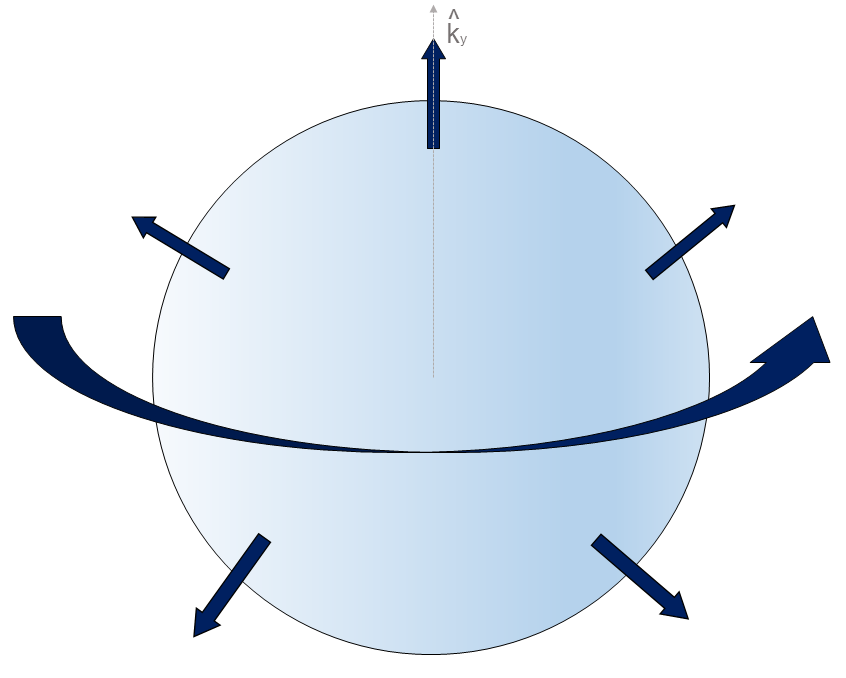
\includegraphics[width=0.6\textwidth]{./figures/chapter2/model}
	\end{center}
	\caption{\textbf{Model:} Spherical LAE with tangential and radial velocity due to rotation and outflows.
		\label{fig:model}}
\end{figure}

These 3 parameters, \vrot, \vout and \tauh, leave the idea of a model of LAE, that although simple, considers the main galaxy's dynamics. All of them have been previously proposed and used by different authors, but never combined together (\cite{Adams72}, \cite{Harrington73}, \cite{Neufeld90}, \cite{Dijkstra06}, \cite{Verhamme06}, \cite{Forero12}, \cite{Martin2015}, \cite{Garavito14}, \cite{Neufeld91}, \cite{Laursen09}, \cite{Barnes11}, \cite{Verhamme12}, \cite{Yajima12}).\\

\section{A \lya Photon's Path in CLARA}
In several problems in science it is useful to define dimensionless variables. This new formulation has many advantages. The numerical equations do not depend on the unit choice. This tends to make the results' analysis straight forward. In the \lya radiative transfer problem, a commonly used dimensionless variable $x$ is used to describe a photon's frequency and is defined as:\\

\begin{equation}
\label{eq:x_freq}
x \equiv \frac{\nu -\nu_{\rm \alpha}}{\Delta\nu_{\rm D}},
\end{equation} 

where $\nu$ is the photon's frequency and $\nu_{\rm \alpha} = 2.46\times 10^{15}$ Hz is the \lya natural frequency. The denominator $\Delta\nu_{\rm D}$ is defined in Eq. \ref{eq:delta_nuD}.

\begin{equation}
\label{eq:delta_nuD}
\Delta\nu_{\rm D} \equiv \nu_{\rm \alpha}\sqrt{\frac{2kT}{m_pc^2}} \equiv \nu_{\rm \alpha} \frac{v_{\rm th}}{c},
\end{equation} 

where $\Delta\nu_{\rm D}$ is known as the Doppler broadening of the \lya line. It depends on the neutral gas temperature $T$ or equivalently the thermal velocity $v_{\rm th}$ of the atoms. In the model the temperature is kept constant at $T=10^4$K and the thermal velocity is $v_{\rm th}=12.8$\kms. \\

If $x < 0$, the final frequency $\nu < \nu_{\rm \alpha}$. This translates to the final wavelength being larger than the \lya natural one. The phenomenon is called a redshift in frequency. If, on the contrary, $x > 0$, the photon suffers a blueshift in frequency. \\

However, in the plots shown in this monograph I use instead velocity, $V$, units. This eases the comparison against observational data. The velocity units are defined by

\begin{equation}
\label{eq:V}
V = xv_{\rm th} = \frac{\nu -\nu_{\rm \alpha}}{\nu_{\rm \alpha}}c.
\end{equation}

The units of $V$ are usually \kms. In this case, the photon is redshifted in frequency when the velocity is greater than 0, and blueshifted in the opposite case. \\

The initial emission of photons is taken at the center of the sphere for practicality due to the fact that both, center and off-center emissions, give analogous results. From here, $100000$ photons are emitted with the natural \lya wavelength. Then, they start to behave as described in section \ref{sec1:laes} (See Fig. \ref{fig:radiative_transfer}). When each photon is re-emitted, its new wavelength depends on the H atom's velocity (both thermal and bulk) and direction (both initial and final). However the photon's new direction of propagation is random in the rest frame of the atom. \\ 

The individual scattering of all the photons is tracked through the complete 3D Hydrogen distribution. Once each photon escapes the galaxy, its final values are stored: position $\vec{r}$, direction of propagation $\hat{k}$, dimensionless frequency $x$, and number of scatterings $N$. To build the observed spectrum I make a histogram of the escape frequencies $x$. The number of scatterings $N$ tells how many steps the random walk requires to reach a distance to the center that is $\geq R$. In order to avoid situations in which the photon has not escaped after a long computational time, CLARA defines a number $N_{max}$ so the code stops. However, according to statistics, this last situation has low probabilities, so the photon is always most likely to exit the sphere. \\

The process that takes place from the moment the first photon is emitted to the moment the last photon escapes the sphere, is called a simulation. Each simulation runs in the scientific computational cluster of Universidad de los Andes due to the computing resources it requires. Depending on \tauh, I need a different number of processors in order to minimize the time demands. For \tauh $=10^5, 10^6, 10^7$ I use 6, 12, 24 processors, respectively. The running times go from 7 hours to 1 week approximately, depending on the case. \\

\section{Galaxy's Viewing Angle}
An observer located far away, only receives photons emitted along its line of sight. That means, only photons escaping in the direction of the observer must be counted in the spectrum. In the simulation I approximate this by taking into account only the photons with escaping direction angle $\theta$ respect to the rotation axis within the range $[\theta_{min}-\theta_{max}]$. I illustrate this in Fig. \ref{fig:viewing_angle_sketch}. \\

\begin{figure}[h!]
	\begin{center}
		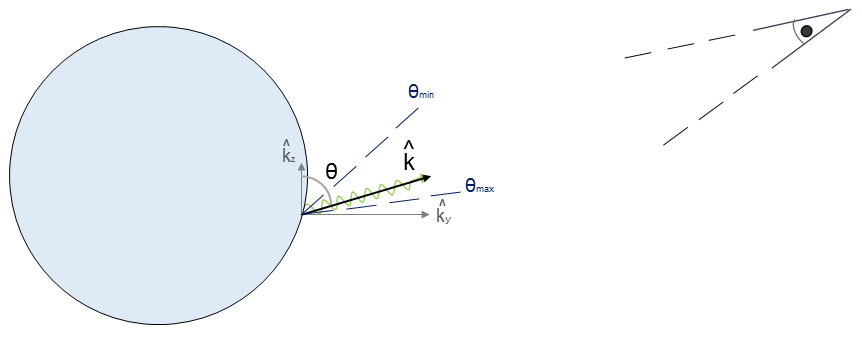
\includegraphics[width=1\textwidth]{./figures/chapter2/viewing_angle_sketch}
	\end{center}
	\caption{\textbf{Viewing Angle Sketch:} The galaxy cut is in the $y-z$ plane perspective and the observer is located at an specific viewing angle of the sphere. Only photons with a direction that enters in this range of vision are taken into account to build the observed spectrum.
		\label{fig:viewing_angle_sketch}}
\end{figure}

Therefore, in principle the spectra depend on two new parameters, the azimuthal and the polar angle. However, the galaxy's motion is symmetrical respect to its rotation axis. This implies that the resulting spectrum is independent from the azimuthal angle. Taking into account this symmetry, I only select photons on their polar angle, regardless of their azimuthal angle. Regarding the polar angle, I build the spectra for observers located on 3 different positions, with $\theta$ intervals uniformly distributed in $\cos(\theta)$. \\ 

To summarize, the parameters influencing the spectra are \vrot, \vout, \tauh and $\theta$. In the next chapter I evaluate the impact each of these has on the resulting profile. 